\section{Proposed \method\ Methodology}
The controller is built in four layers, which are described below in this
order. The problem is first cast as a constrained Markov decision process,
which settles what each role sees and what it controls. A Lyapunov
construction then turns the physical and virtual queues into one reward that
all agents share in every slot. Hybrid MADDPG learns the routing, resource
and flight decisions from this reward, with a deterministic feasibility
controller checking each proposal before it is executed. Last, domain
randomization decides which operating conditions the policy is exposed to
during training.

\subsection{Constrained Markov Decision Process and Agent Roles}
We describe the controller by the tuple
\begin{equation}
\mathcal M=\langle\mathcal S,\{\mathcal O_g\}_{g\in\mathcal G},
\mathcal A,\mathcal P,\mathcal R,\gamma\rangle,
\qquad \mathcal G=\{\mathsf V,\mathsf R,\mathsf U\},
\label{eq:cmdp}
\end{equation}
in which $\mathcal S$ denotes the centralized state space, $\mathcal O_g$ the
observation space of role $g$, $\mathcal A$ the joint hybrid action space,
$\mathcal P$ the transition kernel, $\mathcal R$ the common reward, and
$\gamma\in[0,1)$ the discount factor.

\subsubsection{State and Local Observations}
At the start of slot $t$, the following simulator state is sufficient:
\begin{align}
s_t=\big(&\{Q_j(t)\}_{j\in\mathcal J},
\{\ell_i,\sigma_i(t),b_i^{\rm rem}(t),
c_i^{\rm rem}(t)\}_i,\nonumber\\
&\{\vect p_v(t)\}_v,
\{\vect p_u(t),\vect u_u(t),B_u(t),Z_u(t),m_u(t)\}_u,\nonumber\\
&
\vect c_t,t/T\big),
\label{eq:method_state}
\end{align}
Here $\sigma_i$ is the stage of task $i$, $m_u$ is the activity mode of UAV
$u$, and $\vect c_t$ summarizes the channels and the available resources.
Because the number of tasks varies, task sets are padded up to the configured
maximum and paired with masks. Padding is only a representation device and
never takes a task out of the physical queues.

Actor $h$ of role $g$ receives the observation $o_h(t)=\mathcal O_h(s_t)$. A
vehicle sees its ingress and local workload, the features of its visible
tasks, its position, and the summaries advertised by edge nodes. An RSU sees
its staged and compute queues. A UAV additionally sees its charge, virtual
deficit, return reserve, motion state, nearby agents, and service queues. The
centralized critics are given the full state and the joint action, but only
during training.

\subsubsection{Hybrid Joint Action Space}
With $i_v(t)$ the eligible task at the head of vehicle $v$'s queue, the
actions of the three roles are
\begin{align}
a_v(t)&=\left(h_i,x_i^{L},\{x_{ir}^{R}\}_{r},
\{x_{iu}^{U}\}_{u},\rho_i\right),\nonumber\\
a_r(t)&=\{w_{ir}(t)\}_{i\in\mathcal I_r(t)},\nonumber\\
a_u(t)&=\left(\bar f_u(t),\{w_{iu}(t)\}_{i\in\mathcal I_u(t)},
\vect u_u(t)\right),\nonumber\\
\vect a_t&=\left(\{a_v\}_v,\{a_r\}_r,\{a_u\}_u\right).
\label{eq:joint_action}
\end{align}
A vehicle action is partly categorical (hold the task or pick a destination)
and partly continuous (the UAV-local fraction $\rho_i$). The RSU and UAV
shares lie on a simplex, and the UAV frequency and velocity are continuous
decisions within bounds. Masks that depend on the state remove tasks that do
not exist, nodes without coverage, UAVs that are returning, and destinations
for which no admissible energy contingency is available.

\subsubsection{Transition and Cooperative Reward}
After repair, the executed action $a_t^{\rm exec}=\mathcal H(s_t,\hat a_t)$
leads to
\begin{align}
s_{t+1}&\sim\mathcal P(\cdot\mid s_t,a_t^{\rm exec}),
&r_t&=-G(t),\nonumber\\
J(\pi)&=\E_\pi\!\left[\sum_{t=0}^{T-1}\gamma^t r_t\right].
\label{eq:transition_reward}
\end{align}
Here $G(t)$ is the drift-plus-penalty score, which we define below. Within a
transition, radio and computation service, the movement of tasks between
stages, flight, battery expenditure, end-of-slot harvesting, and new arrivals
are committed in the causal order given in Section~III. All roles get the
same reward, and it is computed from the action that was really executed.

\subsection{Lyapunov Drift-Plus-Penalty Transformation}
\subsubsection{Virtual Net-Energy Deficit}
For every UAV $u$ we introduce the virtual queue
\begin{equation}
Z_u(t+1)=\left[Z_u(t)+E_u(t)-H_u(t)-\bar e_u\right]^+,
\label{eq:virtual_energy_correct}
\end{equation}
where $E_u(t)$ is the energy actually spent, $H_u(t)$ is the replenishment
realized at the end of the slot, and $\bar e_u$ is the average net draw that
is permitted. The physical charge is still governed by the battery-causality
equations of Section~III. $Z_u$ only keeps account and cannot supply any
energy.

With fixed scales $Q^*>0$ and $E^*>0$, we define the normalized quantities
\begin{align}
q_j&=Q_j/Q^*, & z_u&=Z_u/E^*,\nonumber\\
y_j&=(A_j-S_j)/Q^*,
&e_u&=(E_u-H_u-\bar e_u)/E^*.
\end{align}
We take a quadratic Lyapunov function, whose conditional drift is
\begin{align}
L(t)&=\frac12\sum_jq_j^2(t)+\frac12\sum_uz_u^2(t),\nonumber\\
\Delta_L(t)&=\E[L(t+1)-L(t)\mid s_t].
\end{align}
Applying the standard inequality for a squared positive part, we obtain
\begin{align}
\Delta_L(t)+V\E[C(t)\mid s_t]
&\le D_0+\E[G(t)\mid s_t],\label{eq:dpp_bound_new}\\
G(t)&=VC(t)+w_Q\sum_jq_j(t)y_j(t)\nonumber\\
&\quad+w_Z\sum_uz_u(t)e_u(t),
\label{eq:dpp_score_new}
\end{align}
where $D_0$ does not depend on the action and $C(t)$ is the normalized
instantaneous cost from Section~IV. We set $w_Q=w_Z=1$ in the implementation
except where an ablation says otherwise. When the physical queues are long,
serving work becomes more valuable, and when the virtual deficit is large,
net UAV energy becomes more expensive. The weight $V$ sets the balance
between the immediate cost and the pressure from the backlog.

\begin{figure*}[!t]
\centering
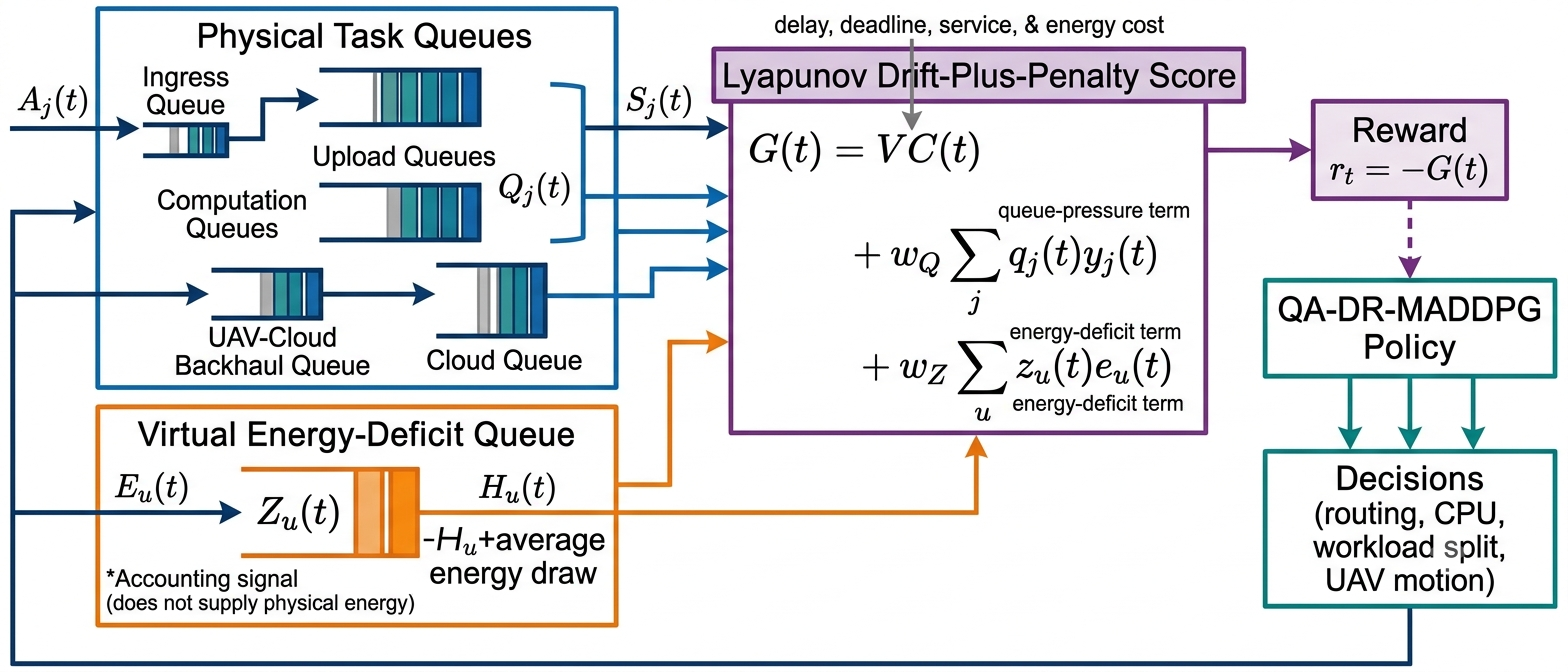
\includegraphics[width=0.94\textwidth]{Physical and virtual queue feedback diagram.png}
\caption{Queue-aware Lyapunov feedback behind the common reward. The
physical task queues and the virtual net-energy deficit both enter the
drift-plus-penalty score, and its negative is passed to the cooperative
controller as the reward. The decisions that are executed then set the queue
service and the energy spent in the next transition.}
\label{fig:lyapunov_feedback}
\end{figure*}

\subsection{Hybrid MADDPG Decision Engine}
The full architecture, with centralized training and decentralized
execution, is drawn in Fig.~\ref{fig:controller_architecture}. Actors shared
within each role form a joint hybrid proposal. The deterministic feasibility
layer turns it into the action that is executed, and the centralized critics
learn from a replay buffer that stores both.

\begin{figure*}[!t]
\centering
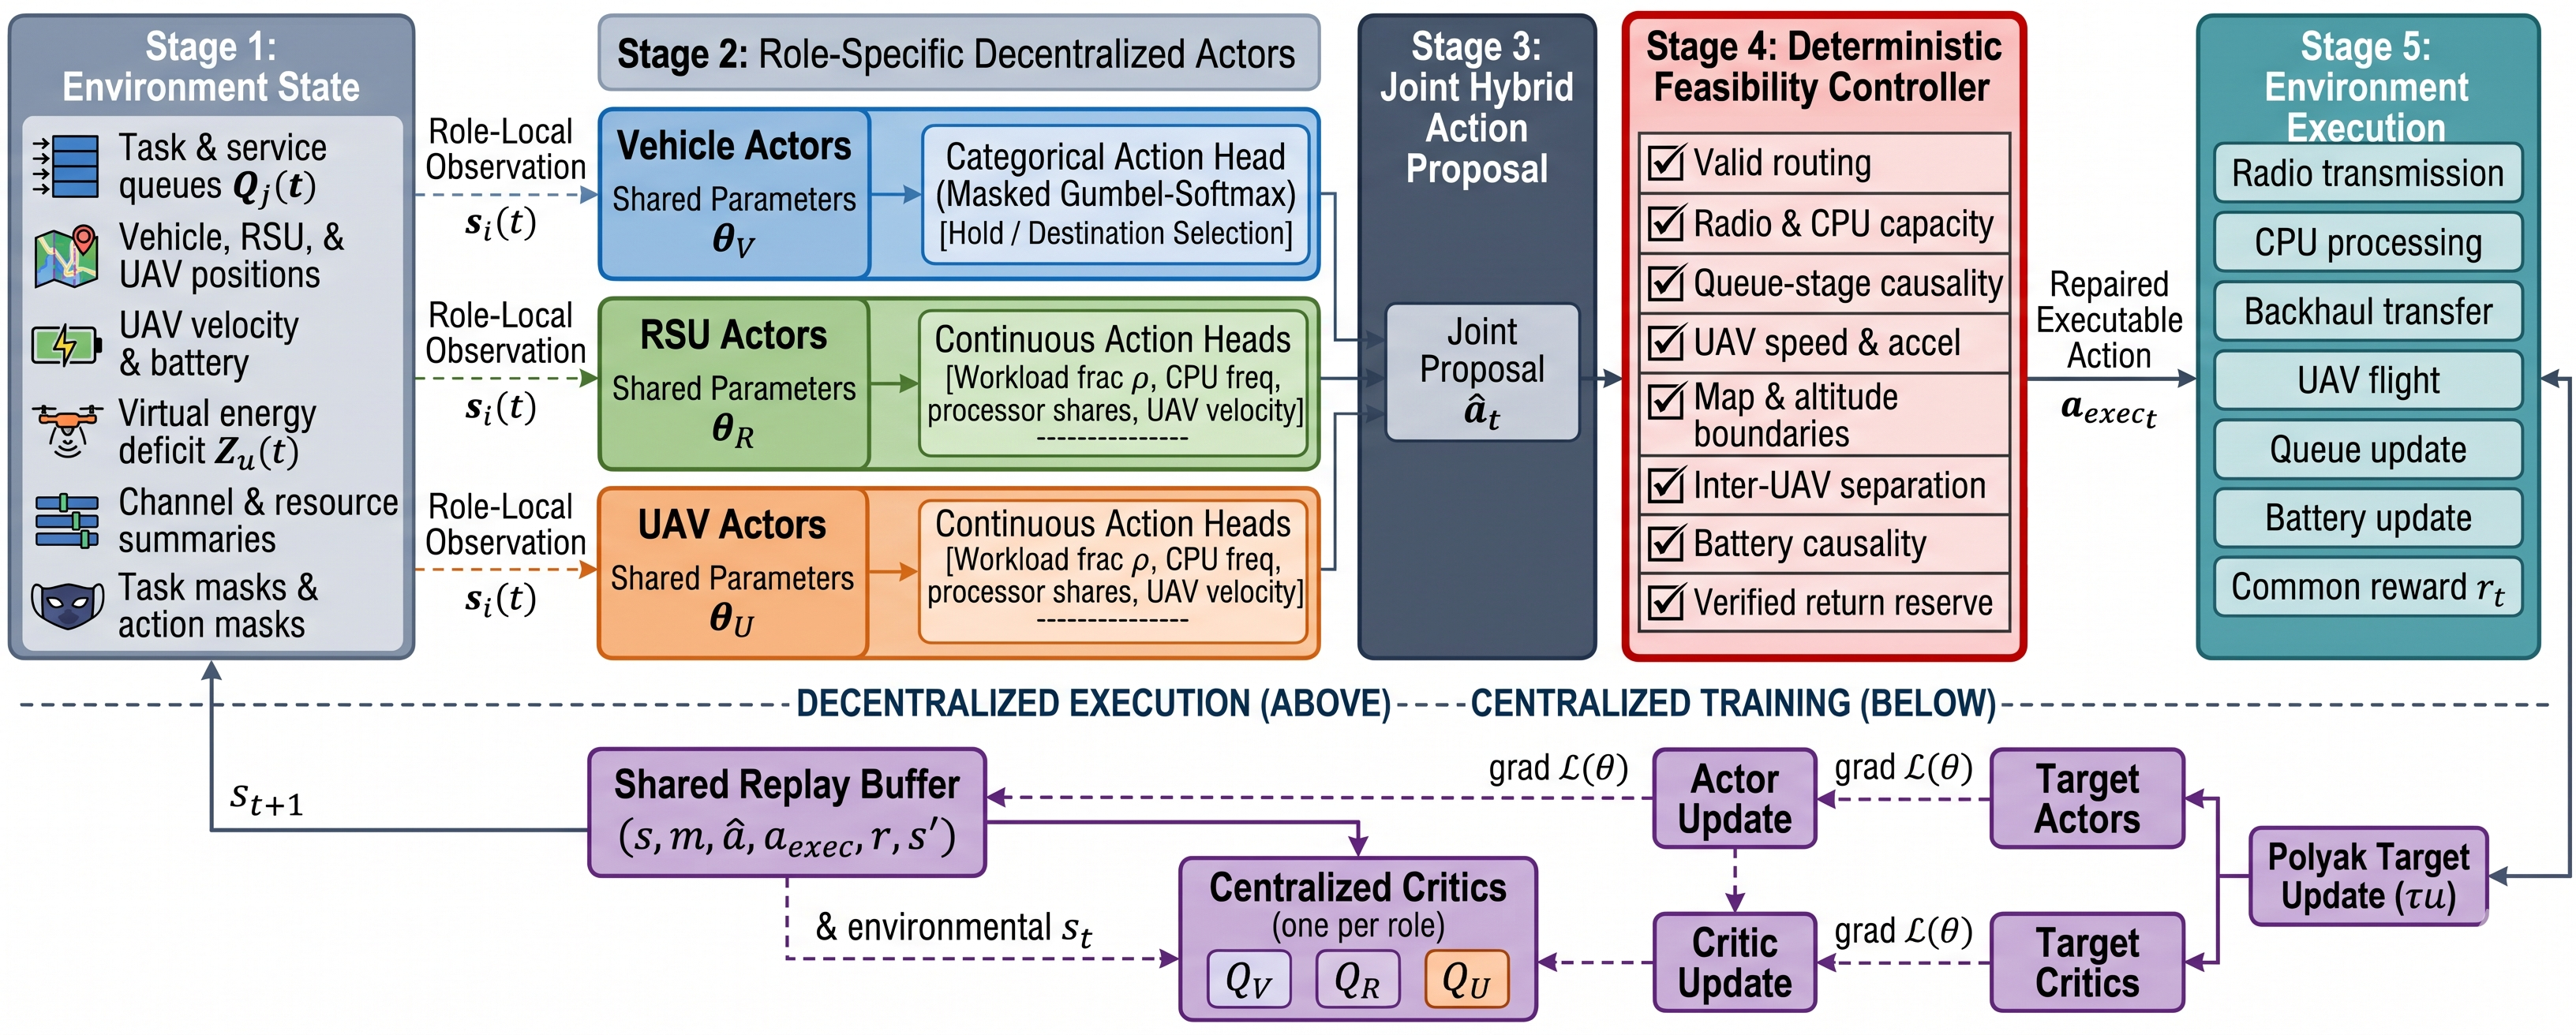
\includegraphics[width=0.98\textwidth]{Complete QA-DR-MADDPG architecture.png}
\caption{Complete \method\ architecture. At execution time, the vehicle,
RSU, and UAV actors rely on role-local observations; the centralized critics
and the shared replay buffer are used only in training. The feasibility
controller sits between the neural proposals and the actions that are
physically executed.}
\label{fig:controller_architecture}
\end{figure*}

\subsubsection{Role-Shared Actors and Centralized Critics}
Each visible task has a feature vector $x_{hi}$ and a mask
$m_{hi}\in\{0,1\}$. The actor passes them through a task encoder followed by
masked pooling:
\begin{align}
e_{hi}&=\phi_g(x_{hi}),\qquad
\bar e_h=\frac{\sum_i m_{hi}e_{hi}}
{\max\{1,\sum_i m_{hi}\}},\nonumber\\
z_h&=\operatorname{LN}\!\left(
\phi_g^{\rm trunk}([o_h;\bar e_h])\right).
\label{eq:actor_encoder}
\end{align}
Parameters are shared by the actors of one role, but different roles have
separate parameters. Each role also has its own centralized critic, which
computes
\begin{equation}
Q_{\psi_g}(s_t,\vect a_t)=q_{\psi_g}([s_t;\operatorname{vec}(\vect a_t)]).
\label{eq:centralized_critic}
\end{equation}

\subsubsection{Categorical and Continuous Action Heads}
Let $l_{hd}$ be the logit of destination $d$ and $c_{hd}$ its feasibility
mask. Choices that are not valid get the logit $-\infty$. In training, the
straight-through Gumbel-softmax output is
\begin{align}
\tilde l_{hd}&=\begin{cases}l_{hd},&c_{hd}=1,\\-\infty,&c_{hd}=0,\end{cases}
\nonumber\\
y_{hd}&=\frac{\exp((\tilde l_{hd}+g_{hd})/\tau_G)}
{\sum_{d'}\exp((\tilde l_{hd'}+g_{hd'})/\tau_G)},\nonumber\\
\hat x_h^{\rm cat}&=\operatorname{sg}
\left(\operatorname{onehot}(\arg\max_d y_{hd})-y_h\right)+y_h,
\label{eq:gumbel_action}
\end{align}
with $g_{hd}=-\log[-\log u_{hd}]$ and $u_{hd}\sim\mathcal U(0,1)$. At
evaluation time there is no Gumbel noise, and the destination is the masked
argmax. The continuous heads are
\begin{align}
\rho_i&=\sigma(z_i^\rho),
&f_u&=f_u^{\max}\sigma(z_u^f),\nonumber\\
\hat{\vect u}_u&=\mathcal S_u\tanh(z_u^{\rm mot}),
&w_{hi}&=\frac{m_{hi}e^{z_{hi}^w}}{\sum_jm_{hj}e^{z_{hj}^w}}.
\label{eq:continuous_heads}
\end{align}
These forms keep the partition fraction and the frequency bounded, keep each
motion component within its configured limit even before physical repair,
and make the positive task shares add up to one.

\subsubsection{Feasibility Controller}
The candidate set $\mathcal C(s_t,\hat a_t)$ holds the proposal itself,
scaled versions of its motion, and the verified contingencies. From it, the
executable action is chosen as
\begin{equation}
a_t^{\rm exec}=\mathcal H(s_t,\hat a_t)
\in\arg\min_{a\in\mathcal C(s_t,\hat a_t)\cap\mathcal F(s_t)}
D(a,\hat a_t),
\label{eq:feasibility_projection}
\end{equation}
where the distance $D$ combines the disagreement in the categorical choices
with the normalized distance between the continuous values. Membership in the
feasible set requires the routing masks, radio and CPU capacity, stage
causality, the speed and acceleration limits, the map and altitude limits,
separation along the continuous path, battery causality, and the return
reserve to be respected. When normal service is not admissible, the UAV stops
accepting new work and follows a verified return or landing contingency. We
keep a record of how proposals differ from the executed actions and of how
often repairs occur, and use both in the evaluation.

\begin{figure*}[!t]
\centering
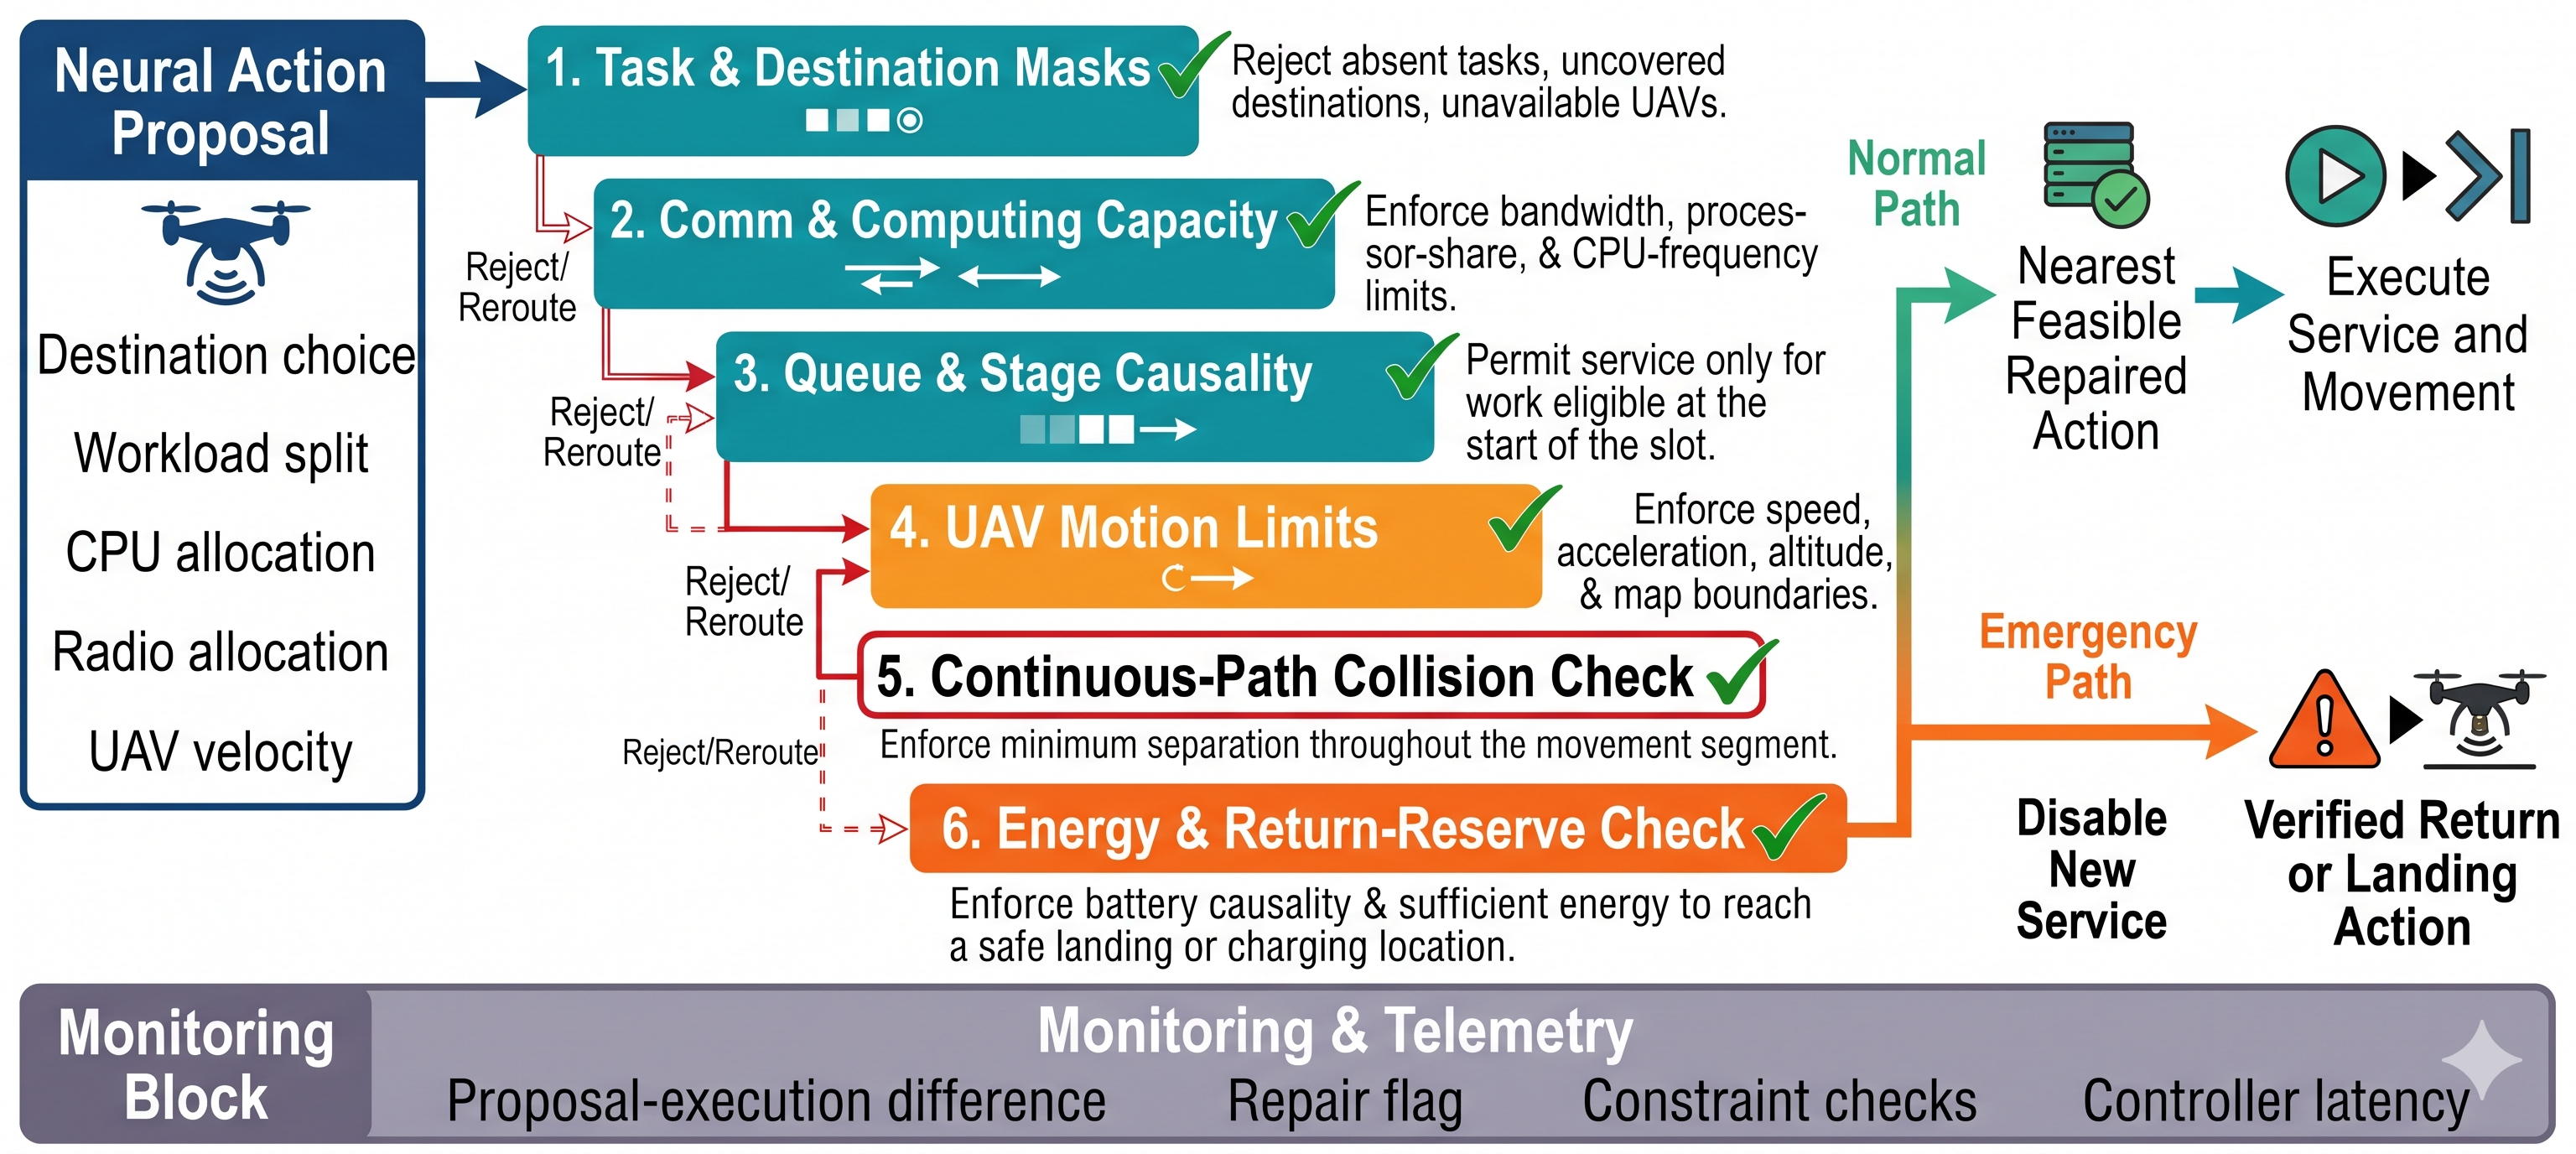
\includegraphics[width=0.95\textwidth]{Feasibility controller and safe-action workflow.png}
\caption{Workflow of the deterministic feasibility controller. Each hybrid
proposal from the networks is tested against the routing, resource,
queue-causality, motion, continuous-path separation, battery, and
return-reserve constraints. The controller then either executes the closest
admissible repair or triggers a verified return or landing contingency.}
\label{fig:feasibility_workflow}
\end{figure*}

\subsubsection{Critic, Actor, and Target Updates}
Each replay entry holds the current and next states, the role observations,
the masks, the proposed and executed joint actions, the reward, and the done
flag $d_b$. For a minibatch of size $B$, the target and the critic loss are
\begin{align}
y_{g,b}&=r_b+\gamma(1-d_b)Q_{\psi_g^-}
(s'_b,\mathcal H_{\rm tens}(\vect a'_b)),\label{eq:critic_target_new}\\
\mathcal L_g(\psi_g)&=\frac1B\sum_{b=1}^{B}
\left(Q_{\psi_g}(s_b,a_b^{\rm exec})-y_{g,b}\right)^2.
\label{eq:critic_loss_new}
\end{align}
When the actor of role $g$ is updated, its current proposal is combined with
the executed replay actions of the other roles, which are detached from the
gradient. Writing $\tilde a_b^{(g)}$ for this mixed action, the actor
maximizes
\begin{equation}
J_g=\frac1B\sum_bQ_{\psi_g}(s_b,\tilde a_b^{(g)})
-\lambda_{\rm rep}\frac1B\sum_b
\|\hat a_{g,b}-\operatorname{sg}(a_{g,b}^{\rm exec})\|_2^2.
\label{eq:actor_objective_new}
\end{equation}
The repair term pulls proposals toward actions that can really be executed.
We do not differentiate through the full physical controller. Following the
Adam updates, the target networks are moved by
\begin{equation}
\theta_g^-\leftarrow(1-\tau_p)\theta_g^-+\tau_p\theta_g,
\qquad
\psi_g^-\leftarrow(1-\tau_p)\psi_g^-+\tau_p\psi_g.
\label{eq:polyak_new}
\end{equation}
In the configuration we report, one actor--critic update is made after every
environment transition as soon as the replay buffer holds 64 samples or more.

\subsection{Domain-Randomized Training and Deployment}
In the completed study, a scenario domain is the tuple
\begin{equation}
\omega=(\lambda,H,C^{\rm bh},\xi),
\label{eq:domain_tuple_correct}
\end{equation}
in which $\lambda$ sets the load or a change in traffic, $H$ selects nominal,
zero, or interrupted replenishment, $C^{\rm bh}$ is the backhaul capacity,
and $\xi$ is the recorded random seed for tasks and harvesting. There are
$10\times7=70$ scenario specifications in the training manifest. In each
epoch, seven different specifications are drawn from it uniformly and
without replacement. In expectation, every declared stress class is seen
equally often, although a given epoch need not contain an example of each
class.

We train for the robust objective
\begin{equation}
\max_\Theta\;\E_{\omega\sim p_{\rm train}}
\E_{\tau\sim\pi_\Theta,\omega}
\left[\sum_{t=0}^{T-1}\gamma^t r_t\right].
\label{eq:dr_objective_new}
\end{equation}
Every episode updates the same parameters $\Theta$. No task-specific copies
are made, and there is no Reptile interpolation. Validation is done on 35
separate specifications (five seeds for each of the seven stresses). A
checkpoint is kept only if it raises the mean validation reward and has zero
modeled physical violations. For early stopping, the patience is ten
validations.

\begin{figure*}[!t]
\centering
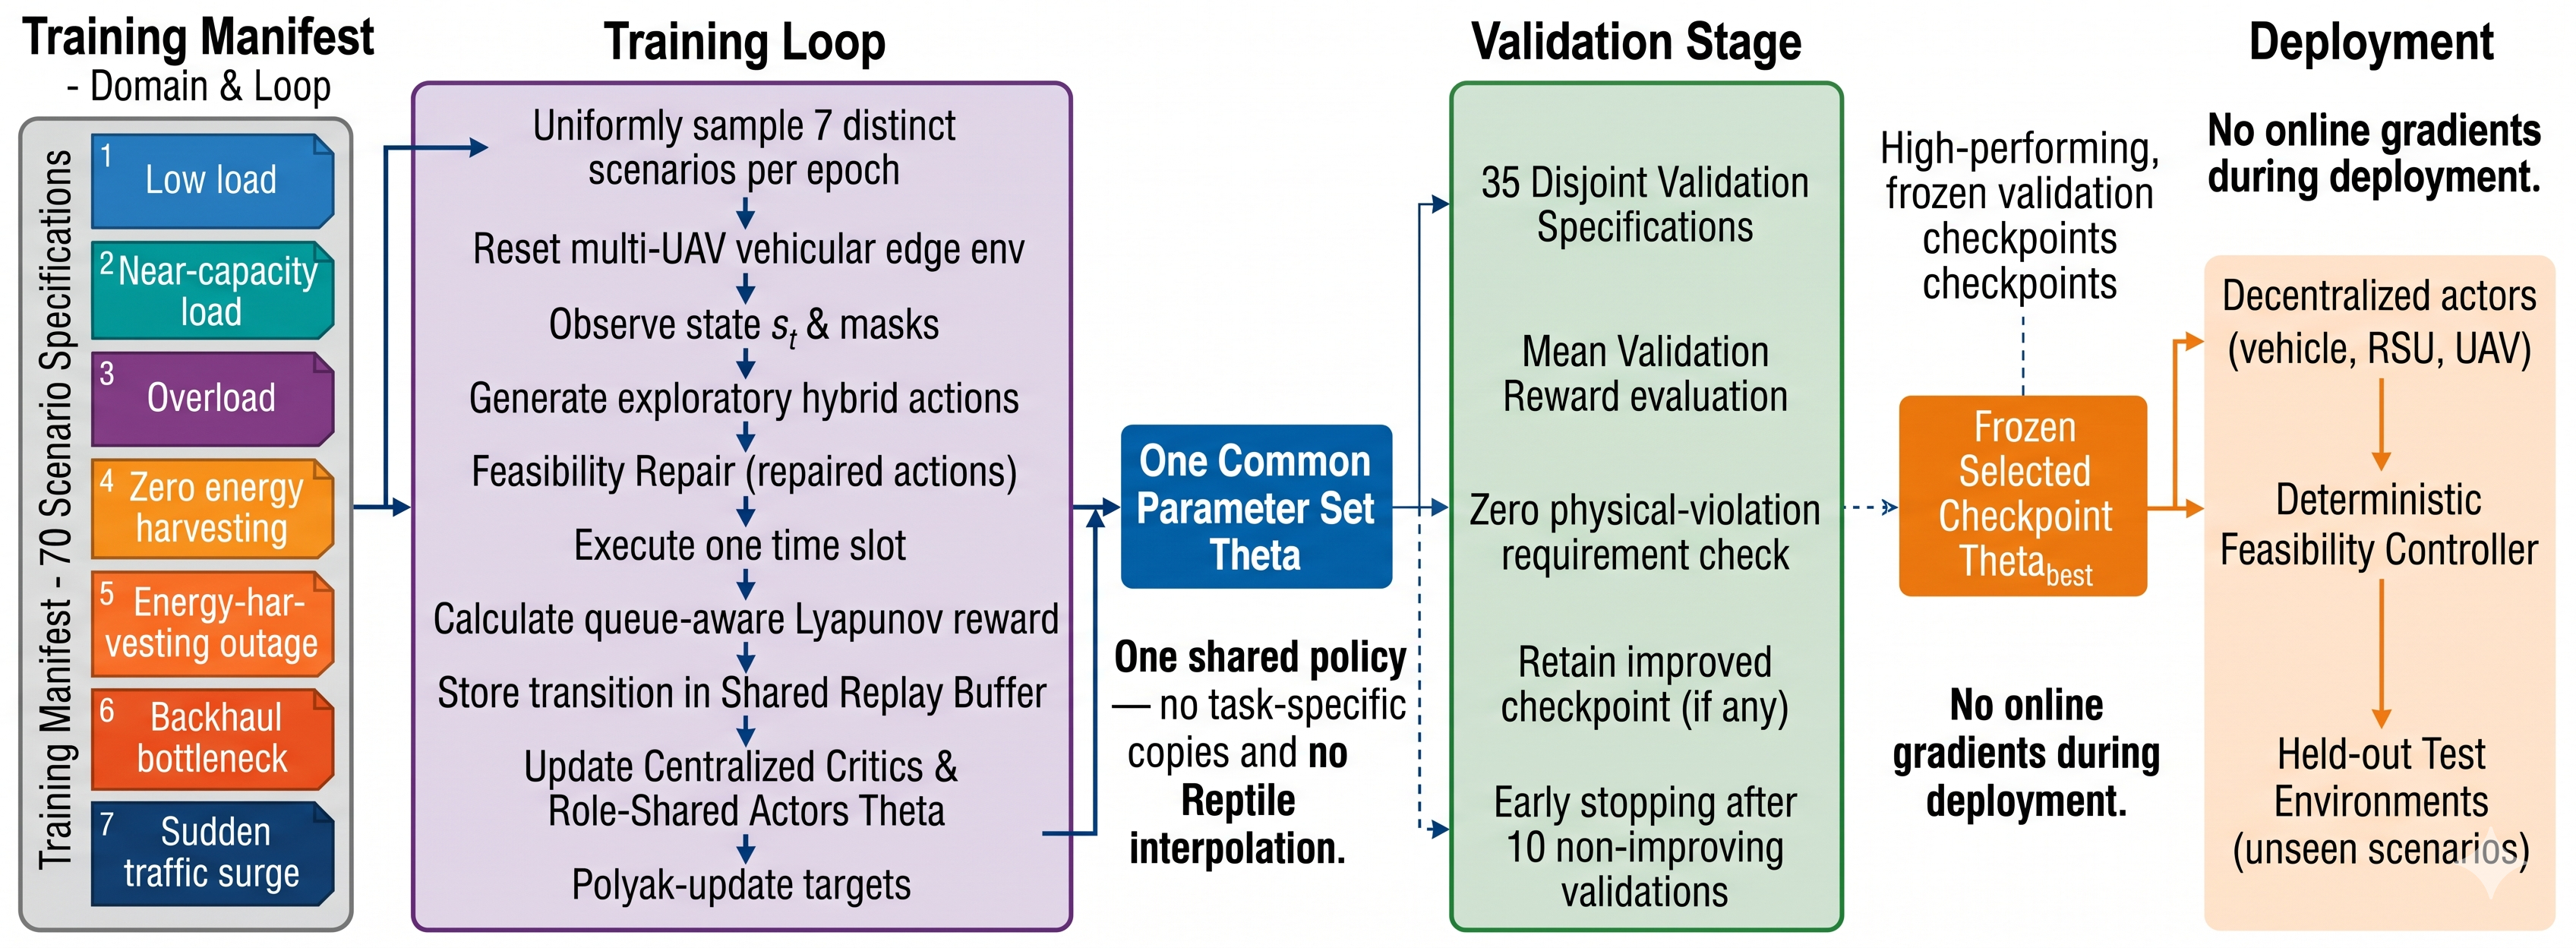
\includegraphics[width=0.98\textwidth]{Domain-randomized training and deployment workflow.png}
\caption{Workflow for domain-randomized training, validation, and
deployment. All seven stress classes update a single shared set of
parameters, and validation on separate data picks an improved checkpoint
with no violations. At deployment, the selected actors are frozen, and the
centralized critics, replay sampling, and gradient updates are switched off.}
\label{fig:dr_workflow}
\end{figure*}

\begin{algorithm}[!t]
\caption{Queue-aware domain-randomized Hybrid MADDPG}
\label{alg:dr_maddpg_new}
\KwIn{Training manifest $\Omega_{\rm tr}$, replay capacity $N$, batch size $B$,
target rate $\tau_p$}
\KwOut{Validation-selected parameters $\Theta^*$}
Initialize online/target actors, critics, and replay $\mathcal D$\;
\For{each epoch $e$}{
 sample seven distinct scenarios $\omega\subset\Omega_{\rm tr}$\;
 \For{each sampled scenario and slot $t$}{
  encode $s_t$, local observations, task masks, and action masks\;
  generate exploratory hybrid proposal $\hat a_t$\;
  execute $a_t^{\rm exec}=\mathcal H(s_t,\hat a_t)$\;
  observe $r_t,s_{t+1}$ and append the complete transition to $\mathcal D$\;
  \If{$|\mathcal D|\ge B$}{
   update all role critics using Eq.~\eqref{eq:critic_loss_new}\;
   update all role actors using Eq.~\eqref{eq:actor_objective_new}\;
   apply Eq.~\eqref{eq:polyak_new}\;
  }
 }
 evaluate the fixed policy on all validation specifications\;
 retain only an improved, zero-violation checkpoint; stop after ten
 non-improving validations\;
}
\end{algorithm}

Once deployed, the controller needs, in each slot, one forward pass through
the role-local actors and then a call to the deterministic feasibility
controller. The selected parameters do not change, since the centralized
critics, replay sampling, and gradient updates are all disabled. What the
evaluation measures, then, is how well the trained policy generalizes to the
test scenarios with no online adaptation.

\subsection{Computational and Storage Complexity}
For role $g$, let $n_g$ be the number of agents, $d_g$ the observation width,
and $a_g$ the action width. We also write $M_{\rm task}$ for the maximum
number of visible tasks, $d_{\rm task}$ for the width of a task feature,
$h_a$ and $h_c$ for the hidden widths of the actor and the critic, $d_s$ for
the width of the global state, and $d_A=\sum_gn_ga_g$. One joint pass
through the actors then costs
\begin{align}
C_\mu=\mathcal O\!\Bigg(\sum_gn_g\big[&
M_{\rm task}(d_{\rm task}h_a+h_a^2)\nonumber\\
&+(d_g+h_a)h_a+h_a^2+h_aa_g\big]\Bigg),
\label{eq:actor_complexity_new}
\end{align}
and with one centralized critic per role, the critic cost is
\begin{equation}
C_Q=\mathcal O\!\left(|\mathcal G|
\left[(d_s+d_A)h_c+h_c^2+h_c\right]\right).
\label{eq:critic_complexity_new}
\end{equation}
A single minibatch update therefore takes $\mathcal O(B(C_\mu+C_Q))$. If the
feasibility repair tries $K_{\rm rep}$ joint candidates, each at cost
$C_{\rm feas}$, it adds at most $\mathcal O(K_{\rm rep}C_{\rm feas})$ per
slot. The replay buffer needs $\mathcal O(Nd_{\rm tr})$ storage, and the
networks, target networks, gradients, and Adam state together need
$\mathcal O(P_\Theta)$. In decentralized deployment no critic is evaluated,
so the cost per slot is $\mathcal O(C_\mu+K_{\rm rep}C_{\rm feas})$.
